\section{Results}
\label{sec:results}

Our analysis proceeds in steps, each motivated by the limits of the previous one. We first ask which individual models offer the best combination of behavioral and neural prediction, using Pareto fronts. Because these fronts compare models that differ in size and language-modeling quality, we then estimate the association of each constraint with behavioral and neural scores at matched size and perplexity, and use matched model comparisons to locate where these associations come from. Finally, because direct prediction relies on a learned mapping whose capacity grows with model width, we ask whether the same picture holds under representational evaluations that fit no such mapping. Together, these analyses show that, for embeddings, a developmental data budget is associated with better behavioral prediction and a memory constraint with worse neural prediction, that the two constraints do not combine additively, and that neural model rankings depend on the evaluation method.

\subsection{Different models lead behavioral and neural prediction}
\label{sec:results-fronts}

\begin{figure}[t]
\centering
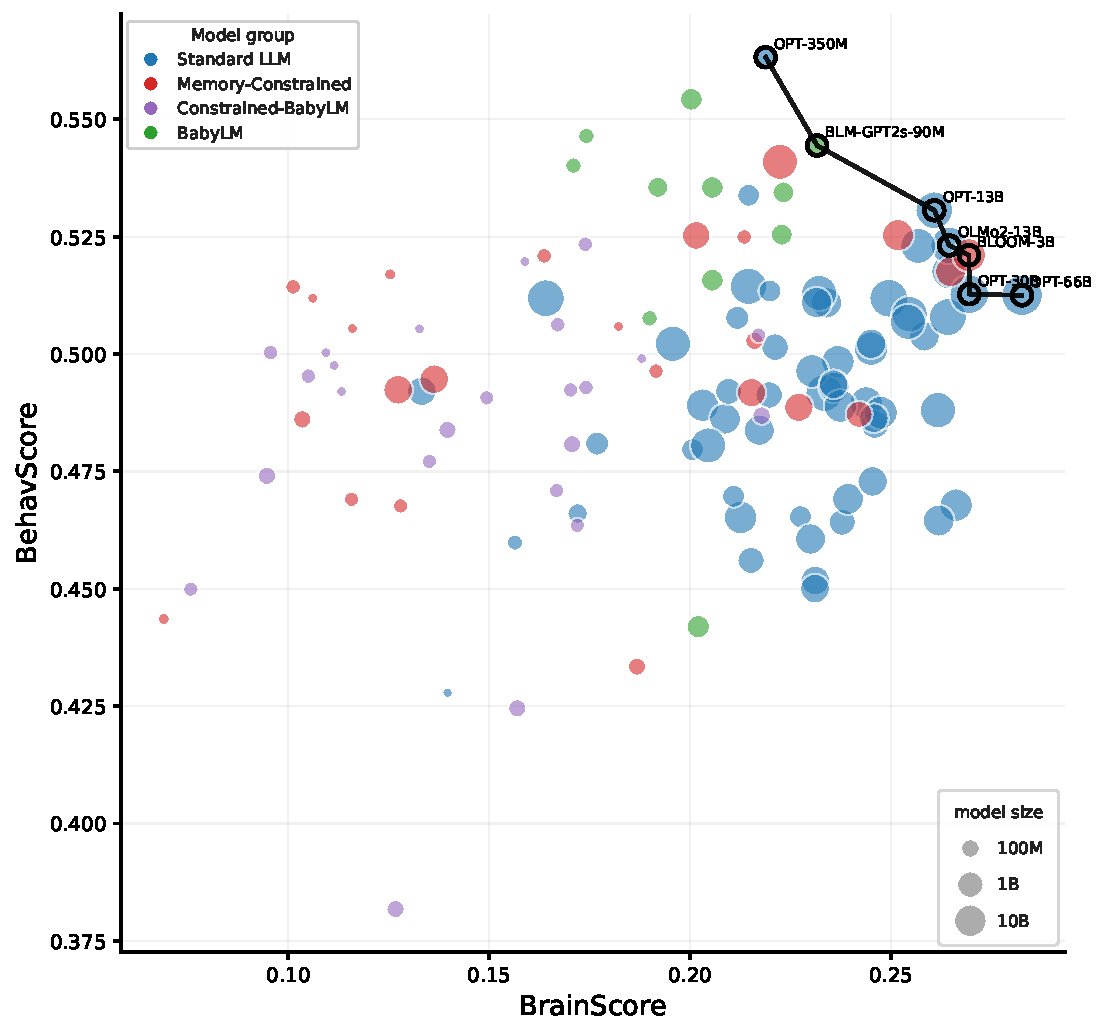
\includegraphics[width=.49\linewidth]{figures/predictive_pareto_embedding.pdf}\hfill
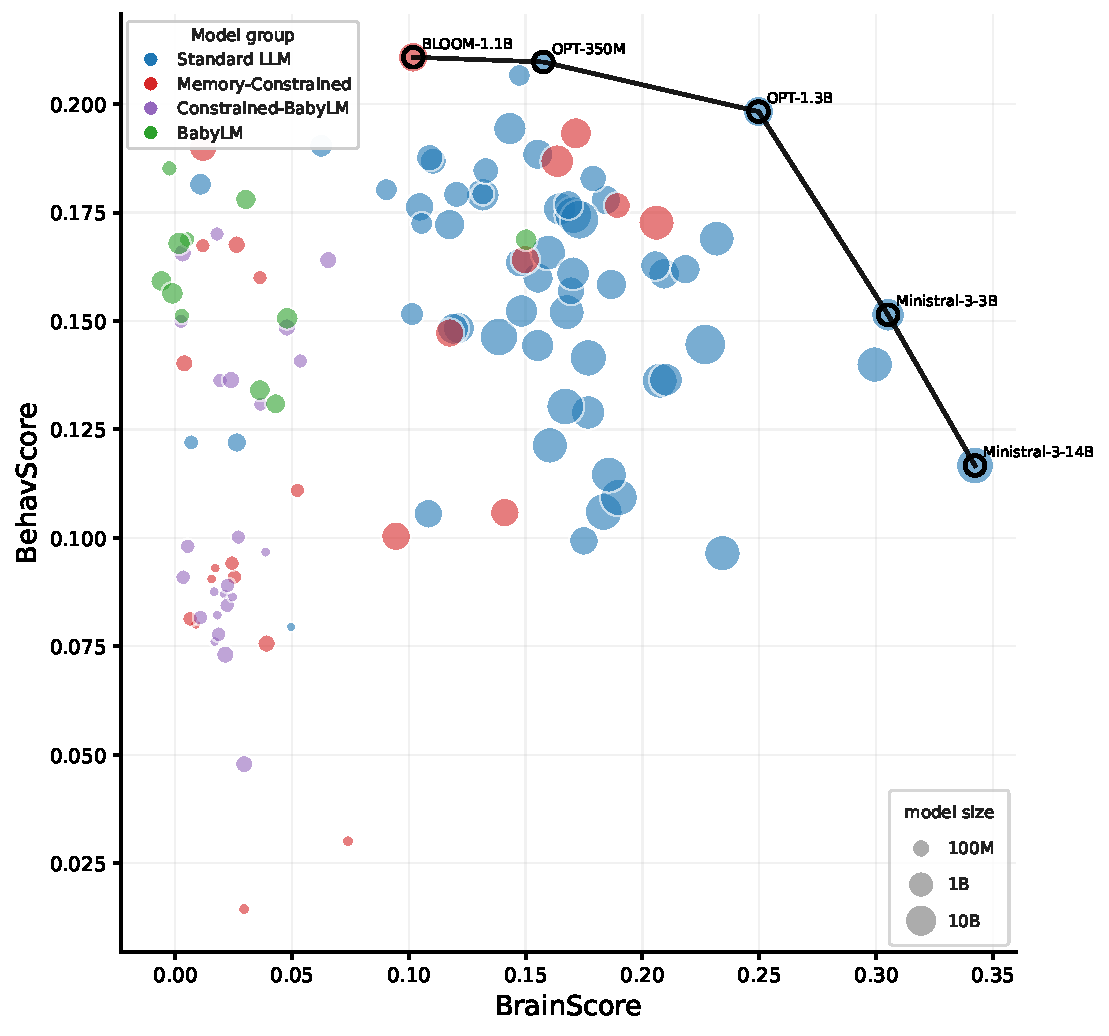
\includegraphics[width=.49\linewidth]{figures/predictive_pareto_surprisal.pdf}
\caption{Direct-prediction Pareto fronts for final-layer embeddings (left) and surprisal (right). Axes are medians of ceiling-normalized dataset-unit scores. Colors identify model groups and marker sizes encode parameter count on a logarithmic scale. Black outlines identify nondominated models. The two tracks have different score definitions; their axis values are not directly comparable.}
\label{fig:predictive-pareto}
\end{figure}

To obtain a first overview of how the 118 models trade off behavioral and neural alignment, we plot each model's BehavScore against its BrainScore and identify the Pareto front, i.e.\ the models that no other model outperforms on both axes at once. No evaluated model maximizes both behavioral and neural scores in either feature track (Figure~\ref{fig:predictive-pareto}). Standard LLMs occupy most frontier positions, alongside specific constrained models. The embedding frontier contains five Standard LLMs, BLM-GPT2s-90M from BabyLM, and the memory-constrained BLOOM-3B. Its behavioral endpoint is OPT-350M, while OPT-66B has the highest neural composite. The surprisal frontier contains four Standard LLMs and BLOOM-1.1B: BLOOM-1.1B leads behavior, whereas Ministral-3-14B leads the neural composite. Neither direct-prediction frontier contains a Constrained-BabyLM model. The models that lead behavioral prediction are thus different from, and typically much smaller than, those that lead neural prediction, a first indication that the two domains reward different model properties.

These fronts identify competitive individual models, but they do not tell us whether a constraint is associated with better or worse alignment as a group. To address this question, we first compare group medians directly.

\subsection{Unadjusted differences between groups}
\label{sec:results-raw}

\begin{table}[t]
\centering
\small
\caption{Unadjusted group medians of the composite scores (median across models within a group of each model's BehavScore or BrainScore; last layer, ceiling-normalized). $N$ is the number of models with at least one finite score. These raw differences confound the constraints with size and perplexity; Table~\ref{tab:main-regression} adjusts for both.}
\label{tab:medians}
\begin{tabular}{lrrrrr}
\toprule
& & \multicolumn{2}{c}{Embeddings} & \multicolumn{2}{c}{Surprisal}\\
\cmidrule(lr){3-4}\cmidrule(lr){5-6}
Group & $N$ & BehavScore & BrainScore & BehavScore & BrainScore\\
\midrule
Standard LLMs & 59 & 0.492 & 0.232 & 0.161 & 0.143\\
Memory-Constrained & 24 & 0.504 & 0.185 & 0.126 & 0.055\\
BabyLM & 11 & 0.535 & 0.202 & 0.159 & 0.030\\
Constrained-BabyLM & 24 & 0.492 & 0.153 & 0.094 & 0.029\\
\bottomrule
\end{tabular}
\end{table}


Table~\ref{tab:medians} gives the median composite score of each group, and it already shows the behavioral--neural asymmetry suggested by the fronts. Standard LLMs have the highest median BrainScore in both tracks, and the gap is large for surprisal (0.143, against 0.055 for Memory-Constrained and about 0.03 for both BabyLM groups). For behavior the ordering differs: with embeddings, BabyLM models have the highest median BehavScore (0.535, against 0.492 for Standard LLMs), and with surprisal, BabyLM and Standard LLMs are close (0.159 and 0.161). Constrained-BabyLM models have the lowest or tied-lowest median in every column. These raw differences do not isolate the constraints, because the groups differ greatly in size, depth and language-modeling quality (Table~\ref{tab:models}). A constrained model could score lower than a Standard LLM simply because it is smaller or a worse language model. To separate the constraints from these factors, we performed a matched-scale analysis: the regressions of Equation~\ref{eq:group}, fit separately for behavioral and neural scores, which compare each group with Standard LLMs of the same size and perplexity.

\subsection{For embeddings, constraints are associated with behavioral and neural prediction in opposite directions}
\label{sec:results-constraints}

\begin{table}[t]
\centering
\small
\caption{Group associations in final-layer direct prediction (Equation~\ref{eq:group}, preferred specification). Coefficients are in noise-ceiling-normalized score units with standard errors in parentheses (Satterthwaite degrees of freedom). Behavioral and neural columns are separate fits with random intercepts for dataset unit, model lineage, model and corpus, and dataset-unit random slopes for size and perplexity. The Neural $-$ behavioral columns come from a joint model of both domains with domain interactions and directly test whether a coefficient differs between them. Single-constraint and combined contrasts are relative to Standard LLMs conditional on parameter count and perplexity. $^*p<.05$, $^{**}p<.01$, $^{***}p<.001$. Robustness checks are in Table~\ref{tab:robustness}.}
\label{tab:main-regression}
\resizebox{\textwidth}{!}{%
\begin{tabular}{lrrrrrr}
\toprule
& \multicolumn{3}{c}{Embeddings} & \multicolumn{3}{c}{Surprisal}\\
\cmidrule(lr){2-4}\cmidrule(lr){5-7}
& Behavioral & Neural & Neural $-$ behav. & Behavioral & Neural & Neural $-$ behav.\\
\midrule
Memory only & $.013\ (.008)$ & $-.031\ (.010)^{**}$ & $-.047\ (.010)^{***}$ & $-.001\ (.008)$ & $-.092\ (.065)$ & $-.089\ (.060)$ \\
Data only & $.033\ (.012)^{**}$ & $-.006\ (.013)$ & $-.042\ (.014)^{**}$ & $.022\ (.011)$ & $-.367\ (.084)^{***}$ & $-.391\ (.079)^{***}$ \\
Memory $\times$ data & $-.040\ (.012)^{**}$ & $.022\ (.014)$ & $.064\ (.015)^{***}$ & $-.026\ (.012)^{*}$ & $.384\ (.092)^{***}$ & $.417\ (.086)^{***}$ \\
Both constraints & $.006\ (.009)$ & $-.016\ (.011)$ & $-.025\ (.011)^{*}$ & $-.005\ (.009)$ & $-.075\ (.072)$ & $-.063\ (.065)$ \\
\midrule
$\log_{10}$ parameters & $.004\ (.003)$ & $.026\ (.012)$ & $.024\ (.010)^{*}$ & $-.035\ (.014)^{*}$ & $.283\ (.192)$ & $.316\ (.159)$ \\
$\log_{10}$ perplexity & $-.005\ (.003)$ & $-.020\ (.009)^{*}$ & $-.009\ (.008)$ & $-.058\ (.024)^{*}$ & $-.105\ (.111)$ & $-.049\ (.095)$ \\
\midrule
Rows / dataset units & 1,822 / 16 & 1,257 / 11 & joint & 1,822 / 16 & 1,257 / 11 & joint \\
\bottomrule
\end{tabular}}
\end{table}


Table~\ref{tab:main-regression} reports the regressions of Equation~\ref{eq:group}. A positive constraint coefficient means that, relative to a Standard LLM of the same size and perplexity, models with that constraint have higher normalized scores in that response domain. Coefficients are in normalized-score units, so their magnitudes are comparable within a column but not across tracks or domains, whose score ranges differ (Appendix~\ref{app:ceiling-values}). Because models of one lineage, scores of one model, and units of one corpus are not independent, the random effects of Equation~\ref{eq:group} widen the standard errors considerably relative to a fit with a dataset-unit intercept only (Appendix~\ref{app:robustness}); we therefore distinguish associations that are robust to the checks described in Section~\ref{sec:design-stats} from those that are not.

We begin with the data constraint in the embedding track, which gives the clearest result. Conditional on size and perplexity, BabyLM models without a memory constraint have higher behavioral embedding scores than Standard LLMs ($\beta_D=.033$, SE $.012$, $p=.008$). This advantage holds in every robustness check, including the lineage bootstrap, the exclusion of the GPT-BERT models, the addition of depth as a covariate, and every leave-one-unit-out refit (Table~\ref{tab:robustness}). On the robust z scale it corresponds to about one between-model standard deviation ($1.05$, 95\% CI $[0.30, 1.81]$), a large difference relative to how much models differ from each other. The corresponding neural contrast is close to zero ($-.006$, SE $.013$), and the joint model confirms that the data contrast differs between the two domains (neural $-$ behavioral: $-.042$, SE $.014$, $p=.007$).

The memory constraint shows the mirror-image pattern. Memory-constrained models have lower neural embedding scores than Standard LLMs of the same size and perplexity ($\beta_M=-.031$, SE $.010$, $p=.002$), an association that also survives every robustness check. Their behavioral embedding contrast is positive but not reliably different from zero ($.013$, SE $.008$, $p=.12$); the advantage that a dataset-intercept-only fit suggests ($.016$, $p<.001$) does not survive modeling the dependence between models. The joint model again shows that the two domains differ ($-.047$, SE $.010$, $p<.001$). For embeddings, the two constraints are thus associated with prediction in opposite directions across the two domains: the data budget with better behavioral prediction, and the memory constraint with worse neural prediction.

Since each constraint alone is associated with an advantage or no difference for behavior, one might expect models combining both to benefit most. The interaction shows the opposite. The memory-by-data interaction for behavioral embeddings is negative ($\beta_{MD}=-.040$, SE $.012$, $p=.002$) and robust, and it cancels the data advantage: Constrained-BabyLM models do not differ from Standard LLMs in either domain ($.006$, SE $.009$, behavioral; $-.016$, SE $.011$, neural).

The surprisal track gives a less clear picture. The behavioral data contrast is positive but marginal ($\beta_D=.022$, SE $.011$, $p=.062$). It is reliable on the robust z scale ($p=.016$) but disappears when UCL self-paced reading, whose likelihood reference is exceeded by many models, is excluded ($.008$, $p=.33$). The neural surprisal contrasts are large in Table~\ref{tab:main-regression} (data only $-.367$, memory $\times$ data $.384$, both $p<.001$), but they are driven by the four units whose likelihood references are flagged as unstable: without them, the data contrast is $-.030$ ($p=.21$) and the interaction $.039$ ($p=.15$). We therefore do not draw conclusions from the neural surprisal constraint coefficients, and treat the surprisal track as inconclusive about the constraints.

\subsection{Design-based comparisons locate the associations}
\label{sec:results-design}

\begin{table}[t]
\centering
\small
\caption{Design-based comparisons. Within architecture: the six memory-limited architectures of \citet{bu2026staticlinearattentionconstraints}, each trained on BabyLM 10M, BabyLM 100M and the Pile at 2 and 4 layers, so that architecture, code and size are fixed and only the training data differ (random intercepts for architecture, model and unit; no size or perplexity adjustment, since perplexity is an outcome of the data). Matched pairs: the two Forgetting Transformer models against their own softmax-attention baselines (mean difference across dataset units; $p$ from a $t$ test across units). By mechanism: the memory-only contrast of Table~\ref{tab:main-regression} estimated separately for each memory mechanism. Coefficients (SE) in normalized score units; $^*p<.05$, $^{**}p<.01$, $^{***}p<.001$.}
\label{tab:design}
\resizebox{\textwidth}{!}{%
\begin{tabular}{lrrrr}
\toprule
& \multicolumn{2}{c}{Embeddings} & \multicolumn{2}{c}{Surprisal}\\
\cmidrule(lr){2-3}\cmidrule(lr){4-5}
& Behavioral & Neural & Behavioral & Neural\\
\midrule
\multicolumn{5}{l}{\textit{Within architecture (36 models; reference: Pile)}} \\
\quad BabyLM 100M & $-.006\ (.005)$ & $.027\ (.010)^{*}$ & $-.005\ (.008)$ & $.052\ (.034)$ \\
\quad BabyLM 10M & $-.012\ (.005)^{*}$ & $.004\ (.010)$ & $-.006\ (.008)$ & $.038\ (.034)$ \\
\multicolumn{5}{l}{\textit{Matched pairs (2 pairs, same data and size)}} \\
\quad Forget gate $-$ softmax baseline & $-.001\ (.004)$ & $-.039\ (.018)$ & $-.004\ (.005)$ & $.006\ (.094)$ \\
\multicolumn{5}{l}{\textit{Memory only, by mechanism (vs Standard LLMs, preferred specification)}} \\
\quad Distance bias (ALiBi, BLOOM) & $.008\ (.014)$ & $-.026\ (.013)$ & $.016\ (.014)$ & $-.109\ (.093)$ \\
\quad Forget gate (Forgetting, FoX) & $.004\ (.011)$ & $-.059\ (.012)^{***}$ & $-.003\ (.011)$ & $-.153\ (.091)$ \\
\quad Stick-breaking (incl.\ MoLM) & $.012\ (.014)$ & $.009\ (.013)$ & $.013\ (.014)$ & $-.100\ (.096)$ \\
\quad Hard $n$-gram window & $.041\ (.014)^{**}$ & $-.016\ (.014)$ & $-.030\ (.014)^{*}$ & $.044\ (.104)$ \\
\quad CBR-RNN & $.037\ (.025)$ & $-.025\ (.023)$ & $.000\ (.032)$ & $.291\ (.176)$ \\
\bottomrule
\end{tabular}}
\end{table}


The group contrasts compare lineages that differ in more than the two binary factors: the memory group pools several mechanisms, and the data contrast compares BabyLM submissions with web-scale LLMs of different architectures. Our model set contains three comparisons that hold more of these differences fixed (Table~\ref{tab:design}), and we used them to ask where the associations come from.

First, the six memory-limited architectures of \citet{bu2026staticlinearattentionconstraints} were each trained on BabyLM 10M, BabyLM 100M and the Pile at two depths, so their training data vary while architecture, code and size stay fixed. Within these architectures, less training data does not improve behavioral prediction: models trained on 10M words predict reading behavior slightly worse from embeddings than the same architectures trained on the Pile ($-.012$, SE $.005$), and 100M-word models do not differ from them ($-.006$, SE $.005$). This agrees with the negative memory-by-data interaction of Table~\ref{tab:main-regression}: for memory-limited architectures, a developmental data budget brings no behavioral benefit. The behavioral data advantage is therefore a contrast between BabyLM-trained standard architectures and web-scale LLMs, which we cannot reduce to the amount of training data alone; it does, however, persist without the six GPT-BERT models (Table~\ref{tab:robustness}), so it is not specific to one BabyLM submission. On the neural side, the 100M-word models predict neural responses from embeddings slightly better than the Pile models ($.027$, SE $.010$), but the 10M-word models do not, so we see no consistent neural dose-response either.

Second, the Forgetting Transformer was released with softmax-attention baselines of the same size, trained on the same data with the same code, giving two matched pairs that isolate the forget gate. The forget gate does not change behavioral prediction in either track, but lowers neural prediction from embeddings ($-.039$, SE $.018$, $p=.058$; lower in eight of eleven neural units). With only two pairs this comparison has little power, but it points in the same direction as the memory contrast of Table~\ref{tab:main-regression}.

Third, estimating the memory contrast separately for each mechanism shows that it is not uniform. The neural embedding penalty comes mainly from forget-gate models ($-.059$, SE $.012$, $p<.001$) and, less clearly, from distance-biased attention ($-.026$, SE $.014$, $p=.055$), whereas stick-breaking attention and hard $n$-gram windows show no neural penalty. Conversely, hard $n$-gram windows are the only mechanism with a behavioral embedding advantage ($.041$, SE $.014$, $p=.006$), the same models that lead the behavioral end of the embedding RSA and RDM-regression fronts; for behavioral surprisal their contrast is negative ($-.030$, SE $.014$). The pooled memory contrast thus averages over mechanisms with different associations, and the neural memory penalty is best described as a property of forget-gate and distance-biased attention.

\subsection{Size and perplexity}
\label{sec:results-scale}

The same regressions show how size and perplexity relate to alignment once group membership is accounted for. In the embedding track, parameter count is positively associated with neural prediction ($.026$ per tenfold increase, SE $.012$, $p=.052$ in the separate fit; $.028$, $p=.002$ in the joint model), and more strongly than with behavioral prediction (neural $-$ behavioral $.024$, SE $.010$, $p=.025$). The size association for neural surprisal is positive but imprecise ($.283$, SE $.192$), reflecting large differences in slope across neural datasets.

For behavioral surprisal, both covariates have negative coefficients: lower perplexity is associated with better prediction ($\beta_Q=-.058$, SE $.024$, $p=.027$), and, at fixed perplexity, larger models predict reading behavior worse ($\beta_S=-.035$, SE $.014$, $p=.025$). Both associations hold in every robustness check, and they are stronger without the flagged UCL unit. Taken together, these findings do not support a universal increase in human alignment with model size: size is associated with better neural prediction from embeddings but, at matched language-modeling quality, with worse behavioral prediction from surprisal.

\subsection{Representational comparisons support behavioral competitiveness and reveal evaluation-dependent neural rankings}
\label{sec:results-rsa}

\begin{figure}[t]
\centering
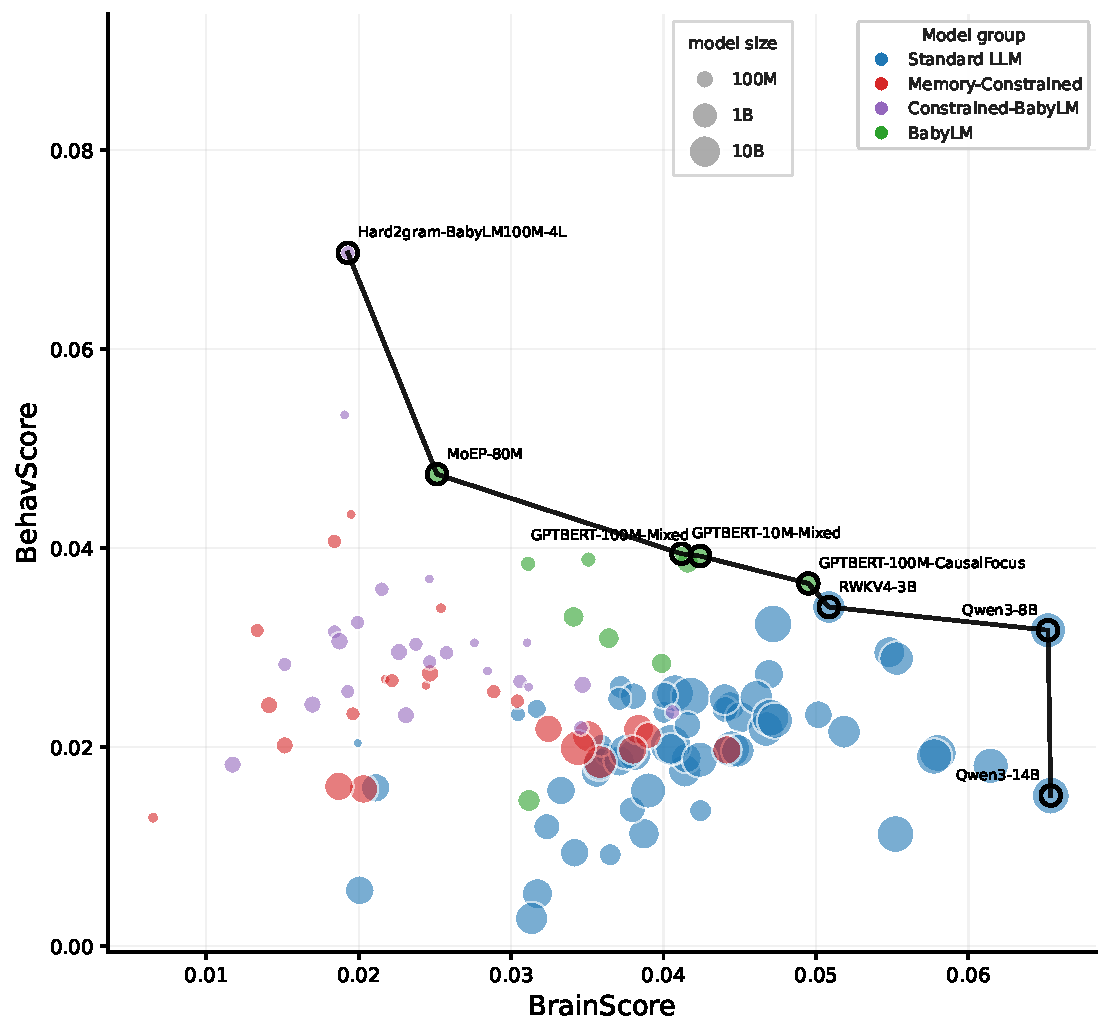
\includegraphics[width=.49\linewidth]{figures/rsa_pareto_embedding_current.pdf}\hfill
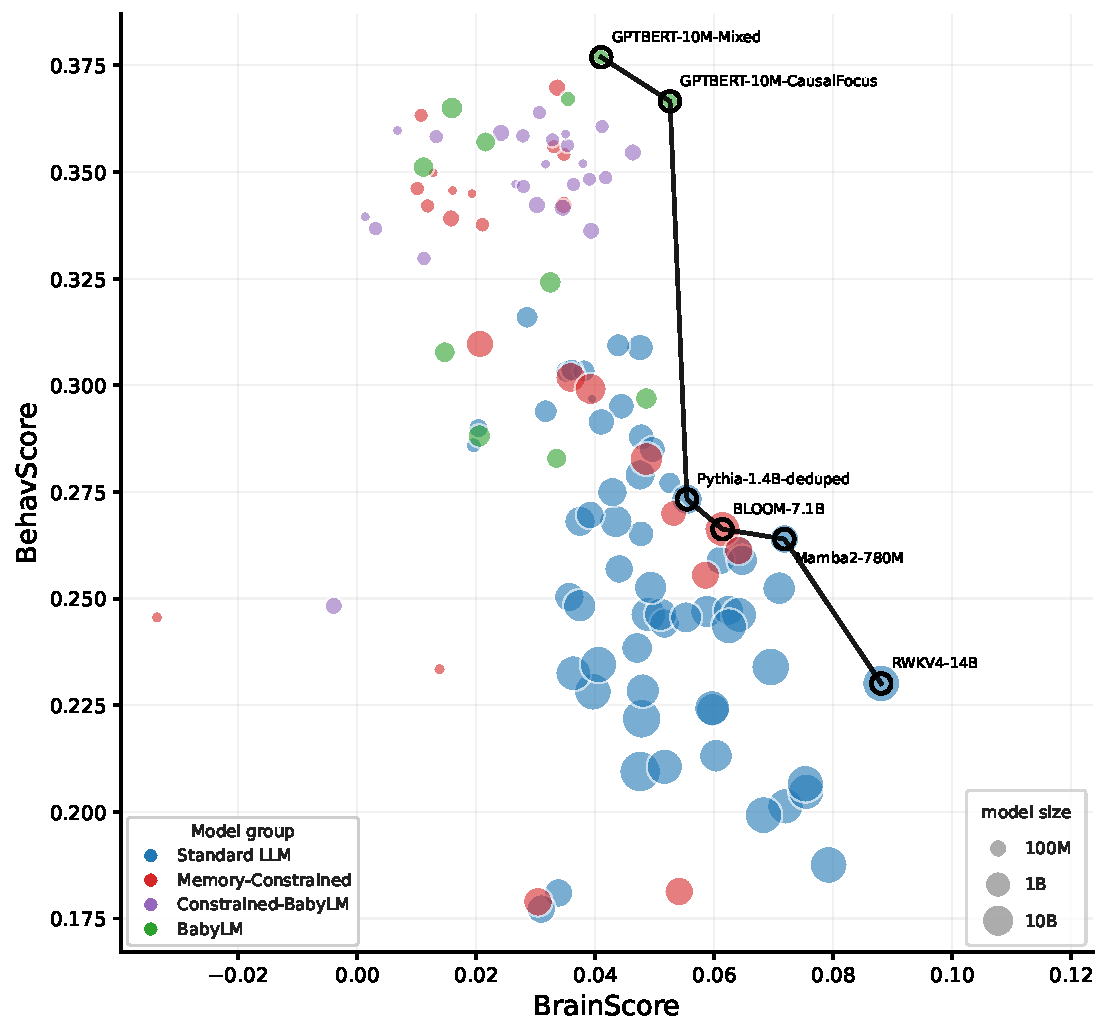
\includegraphics[width=.49\linewidth]{figures/rsa_pareto_surprisal_current.pdf}
\caption{Unfitted Pearson RSA Pareto fronts: embeddings (left) and surprisal (right). Scores summarize model--response RDM correlations divided by their RSA ceilings over eight neural datasets and 16 behavioral measures. Small and constrained models occupy the behavioral end, while Standard LLMs attain the highest neural composites. These descriptive fronts assess representational geometry without fitting a response mapping.}
\label{fig:rsa-pareto}
\end{figure}

The analyses so far rely on direct prediction, in which a learned ridge mapping (for embeddings) or a regression on surprisal relates model features to responses. The capacity of the ridge mapping grows with the width of the representation, which could favor large models for reasons unrelated to representational similarity. To test whether our conclusions depend on this learned mapping, we further performed an unfitted representational similarity analysis, which compares the geometry of model and response dissimilarity matrices directly and assigns every model a single, parameter-free score. The behavioral end of the embedding RSA frontier is occupied by Hard2gram-BabyLM100M-4L, followed by MoEP-80M and GPTBERT models; Qwen3-14B has the highest neural composite (Figure~\ref{fig:rsa-pareto}). For surprisal RSA, GPTBERT-10M-Mixed leads behavior, while RWKV4-14B leads neural alignment. Thus constrained models remain competitive for behavior under an evaluation that does not learn a response mapping. This agrees with the behavioral group findings of the matched-scale analysis, although it is a descriptive convergence rather than an independent adjusted test of the constraint coefficients.

Unfitted RSA, however, does not control for lexical properties: two words may have similar model representations and similar reading times simply because they have similar length or frequency. To rule out this explanation, we additionally fit an RDM regression, which measures how much a model RDM improves held-out prediction of the response RDM beyond word-length and frequency RDMs.

\begin{figure}[t]
\centering
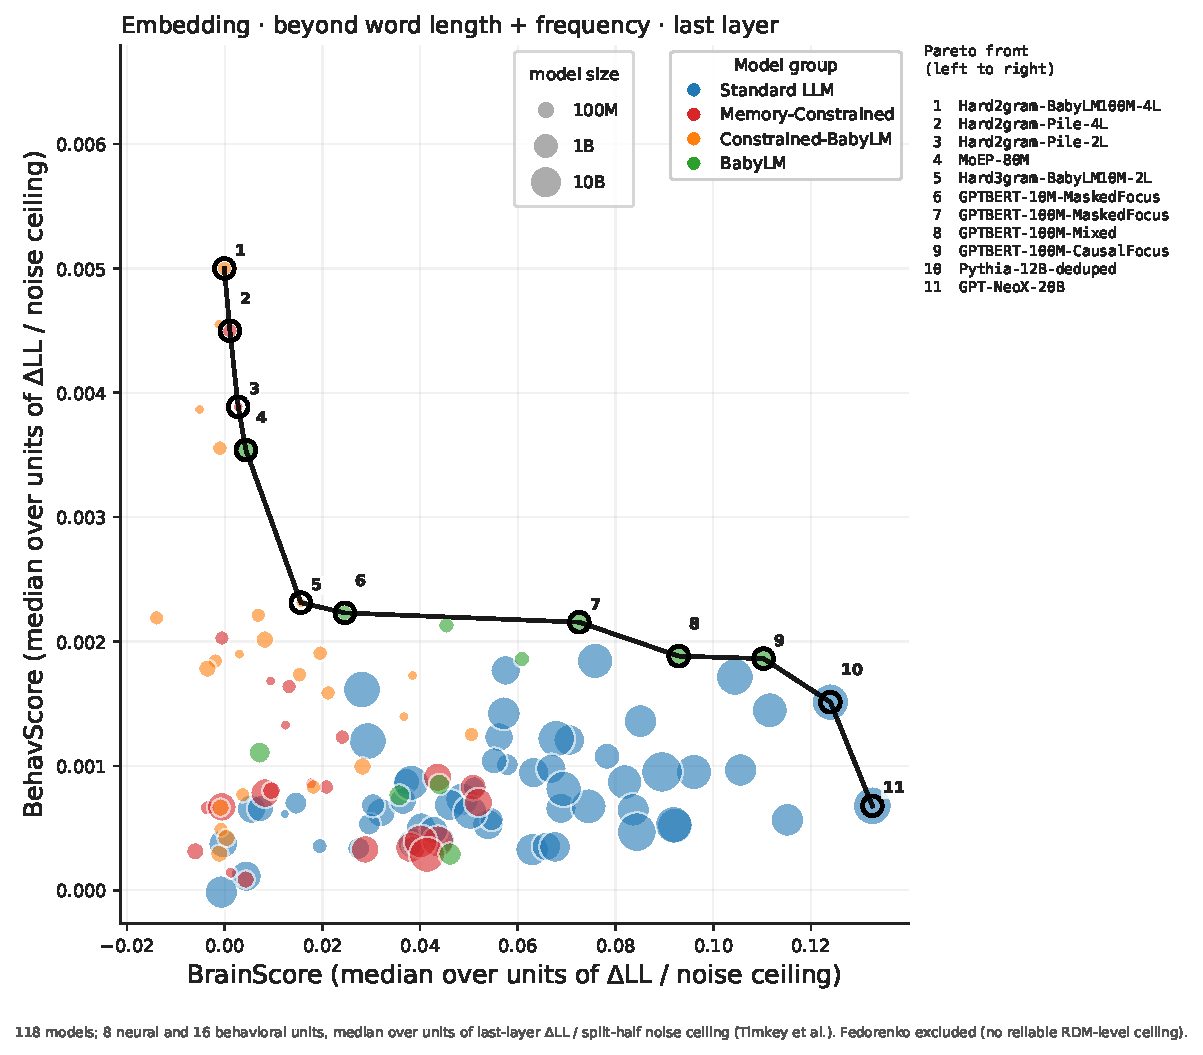
\includegraphics[width=.49\linewidth]{figures/rdm_pareto_embedding_evaluated.pdf}\hfill
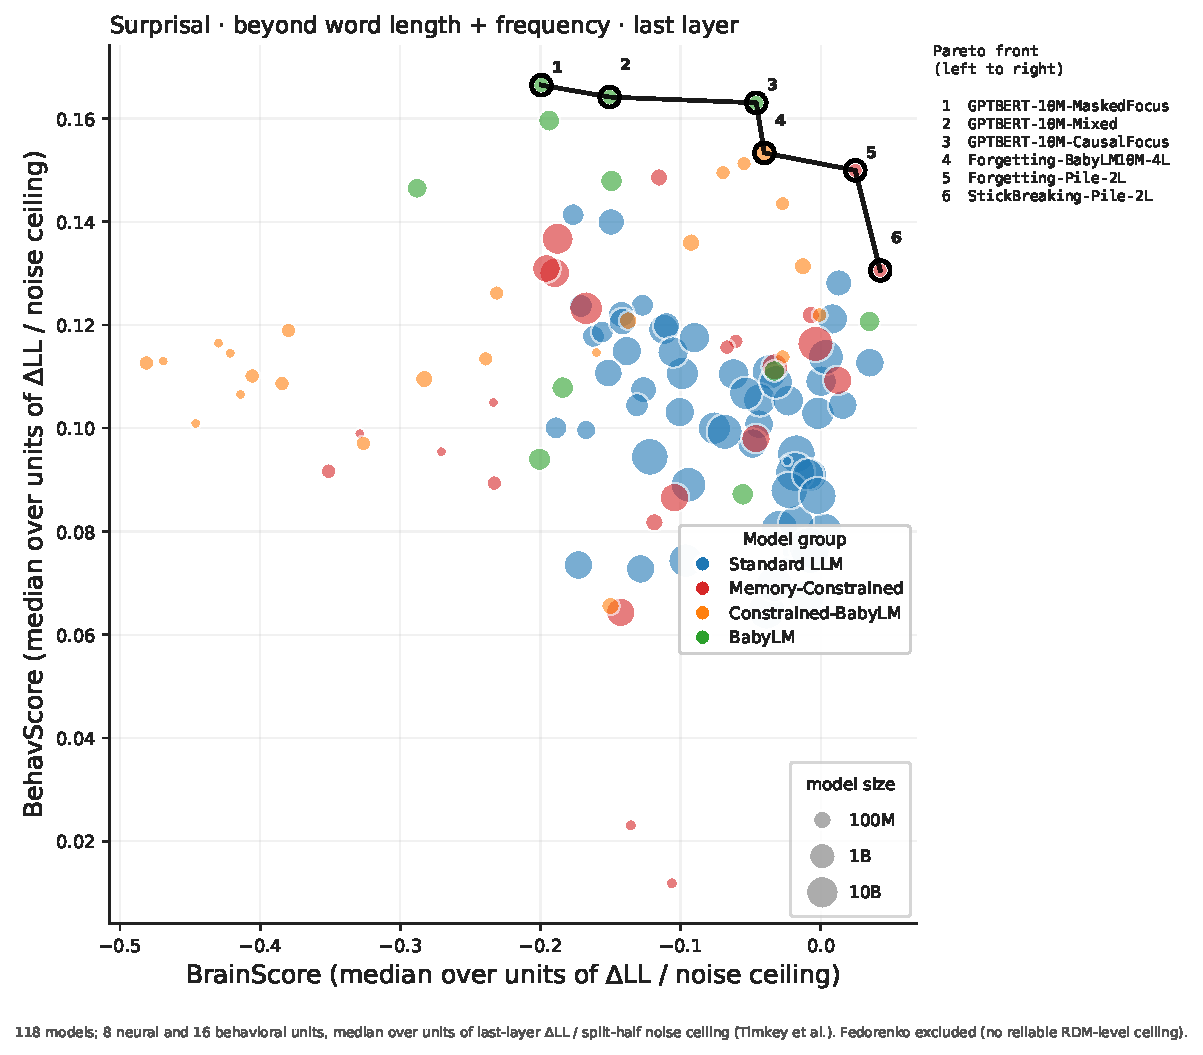
\includegraphics[width=.49\linewidth]{figures/rdm_pareto_surprisal_evaluated.pdf}
\caption{Confound-controlled RDM-regression Pareto fronts: embeddings (left) and surprisal (right). Scores are held-out $\Delta\ell$ per pair beyond word-length and frequency RDMs, divided by split-half references and aggregated across dataset units. Unlike unfitted surprisal RSA, the surprisal regression frontier includes no Standard LLM. Negative scores indicate poorer held-out fit than the confound-only baseline; most neural surprisal scores are negative.}
\label{fig:rdm-pareto}
\end{figure}

Controlling for these lexical distances preserves the behavioral competitiveness of constrained models but changes the neural rankings (Figure~\ref{fig:rdm-pareto}). Because the two axes differ greatly in how much a model RDM adds beyond the lexical baseline, we describe each in turn. For embeddings, the gain on the behavioral axis is small for every model (normalized BehavScores between 0 and .005), whereas most models improve neural prediction beyond the lexical RDMs (BrainScores from $-.014$ to $.133$, positive for 102 of 118 models). The embedding frontier includes all four groups: Hard2gram-BabyLM100M-4L leads behavior, followed by other hard-window and BabyLM models, and BabyLM models also have the highest median behavioral score of the four groups ($.0019$, against $.0007$ for Standard LLMs), while GPT-NeoX-20B leads the neural composite. For surprisal the situation is reversed. Behavioral gains are larger (BehavScores from $.012$ to $.166$), and the frontier consists entirely of BabyLM and constrained models: GPTBERT-10M-MaskedFocus leads behavior, and BabyLM models have the highest median behavioral score ($.147$, against $.103$ for Standard LLMs). On the neural axis, however, surprisal distances add little beyond the lexical RDMs: only 11 of 118 models have a positive BrainScore. The models at the neural end of the frontier, StickBreaking-Pile-2L ($.042$) and Forgetting-Pile-2L ($.025$), are memory-constrained models among these few, but Standard LLMs have the least negative median ($-.049$) and are absent from the frontier only because of their lower behavioral scores. The surprisal results therefore support the behavioral competitiveness of constrained models, but on the neural axis they show a ranking among models that mostly fail to improve on the lexical baseline, not good neural prediction.

Because the matched-scale analysis found opposite size associations for behavioral and neural prediction, we next asked whether representational similarity shows the same domain-dependent scaling. Across the 118 models, embedding RSA correlates positively with log parameter count in seven of eight neural datasets, but negatively in fourteen of sixteen behavioral measures (Table~\ref{tab:rsa-summary}). MEG-MASC is the neural exception ($r=-.558$). Behavioral examples include MECO first-pass duration ($r=-.597$) and ZuCo task-specific reading ($r=-.643$). Because the smallest models are also the constrained ones, these pooled correlations could merely reflect group differences. Within constraint groups (partial correlations controlling for group), the pattern is weaker but keeps its direction: positive in seven of eight neural datasets and negative in twelve of sixteen behavioral measures, with behavioral values mostly between $-.02$ and $-.36$. Surprisal RSA trends are more heterogeneous: correlations with size are positive for the three N400 datasets ($r=.729$--$.795$; $.558$--$.629$ within groups), negative for GECO and OneStop go-past times ($r=-.669$ and $-.813$), and positive for UCL self-paced reading ($r=.507$). These are descriptive associations, not estimates of a universal scaling law (Appendix~\ref{app:rsa-panels}).

Finally, the differences between the direct-prediction and representational fronts raise the question of how closely the two kinds of evaluation agree at the level of individual datasets. We therefore correlated, across models, each dataset's direct-prediction score with its RSA score. Across-model correlations between embedding prediction scores and embedding RSA are positive in all eight available neural datasets ($r=.275$--$.929$), but vary in sign for behavior. They are positive for Provo ($r=.649$--$.678$ across its measures), negative for OneStop first-pass and total dwell times ($r=-.342$ and $-.412$), and close to zero for some other measures. Surprisal comparisons vary in both domains. Among neural datasets, correlations are about $.75$ for Nieuwland and Federmeier 2007, but close to zero or negative for Pereira ($.019$), MEG-MASC ($.138$) and Broderick ($-.119$). Agreement between direct prediction and RSA is thus high only for embeddings on most neural datasets, and even there it is modest for MEG-MASC ($.275$); for behavior, and for surprisal in both domains, it varies in sign. Consequently, good direct prediction does not guarantee the same ranking under representational evaluation. Differences in response construction and coverage also contribute to this comparison.
